\chapter{Program Documentation}
\label{chap:program}

This chapter focuses on the implementation part of the thesis.

\section{Overview}
As mentioned, suggestions are retrieved by a REST API call made to the Web module. This module processes the data and
invokes the Suggester module to return the suggestions. Simplified diagram which shows the main interactions between the
objects and modules can be seen in the Figure \ref{programmer_sequence}.
\begin{figure}[htbp]
    \centering
    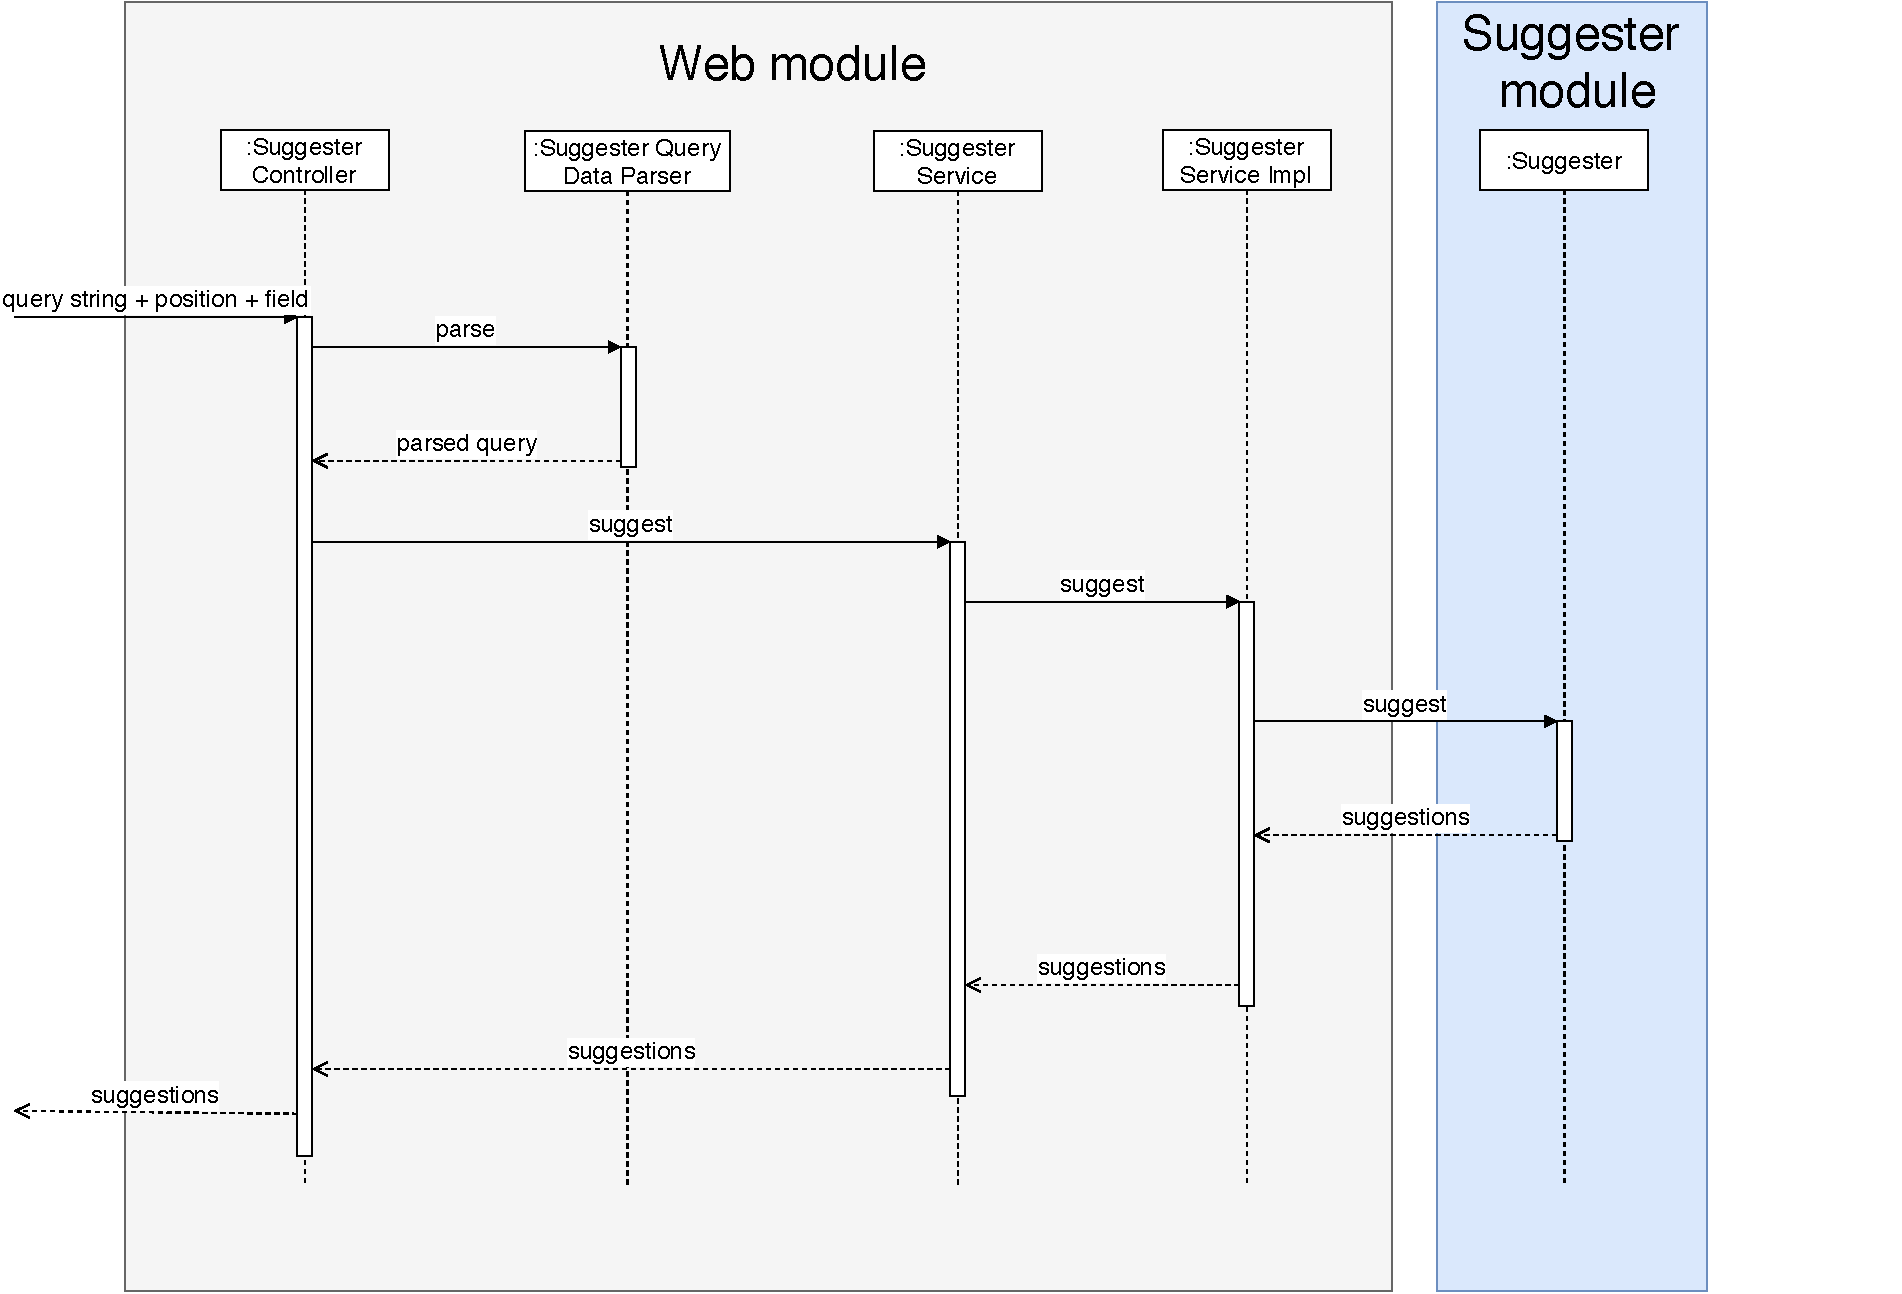
\includegraphics[width=145mm]{../img/programmer_sequence.pdf}
    \caption{Overview of the main object interactions}
    \label{programmer_sequence}
\end{figure}

\section{Web module}
The suggester support was added as a part to the already existing OpenGrok's REST API. The \textit{SuggesterController}
class serves as a REST API endpoint for suggester related queries. Other needed classes are located in the
\textit{org.opensolaris.opengrok.web.api.v1.suggester} package. Classes which are auto-detected by the Jersey
implementation are located in the \textit{org.opensolaris.opengrok.web.api.v1.suggester.provider} package and are annotated
by the \textit{@Provider}\footnote{\url{https://docs.oracle.com/javaee/7/api/javax/ws/rs/ext/Provider.html}} annotation.
The communication with the Suggester module is abstracted in the \textit{SuggesterService} interface and implemented in the
\textit{SuggesterServiceImpl} class. The implementation is injected into the classes which require the
\textit{SuggesterService} by the use of
\textit{@Inject}\footnote{\url{https://docs.oracle.com/javaee/7/api/javax/inject/Inject.html}} annotation. If some other
component which is not part of the REST API part of the application needs to access the \textit{SuggesterService},
it can retrieve it by invoking \textit{getDefault()} method in the \textit{SuggesterServiceFactory} class.

\subsubsection{Configuration Change}
The suggester data structures need to be refreshed on configuration change.
Many basic OpenGrok properties might have changed, for instance:
\begin{itemize}
    \item \textit{dataRoot} which specifies where OpenGrok stores the data.
    \item Suggester configuration.
    \item Projects.
\end{itemize}

It is not trivial to notice all the changes and it would not be feasible from the modifiability point of view to check
specific values for change. Therefore, \textit{SuggesterServiceImpl} closes the underlying suggester data structures
and tries to reinitialize the suggester with the new configuration. If the configuration has not changed in a major
aspect (e.g. different \textit{dataRoot} or new projects were added), then the Suggester module just reloads the data
from disk. Reload from disk should be fast (from the experience less than $1$ s).

\section{Suggester module}
The Suggester module is located under the \textit{suggester} directory of the root of the project. The main class which
exposes the suggester functionality is the \textit{Suggester} class.

\subsubsection{Public API}
\label{public_api}
The public API consists of the following methods:
\begin{itemize}
    \item \textit{init(Collection\textless NamedIndexDir\textgreater)} – initializes all the data structures based on the paths
    to the indexes and their names (project names).
    \item \textit{remove(Iterable\textless String\textgreater)} – removes all the data structures stored for the
    specified names.
    \item \textit{search(List\textless NamedIndexReader\textgreater, SuggesterQuery, Query)} –
    searches the suggester data and returns suggestions to the provided queries.
    \item \textit{onSearch(Iterable\textless String\textgreater, Query)} –
    event signalization that the query was searched. Updates the data structures for the most popular completion.
    \item \textit{increaseSearchCount(String, Term, int)} – updates the search count for the specified project and term by the
    specified int value. Negative values are not allowed.
    \item \textit{getSearchCounts(String, String, int, int)} – returns popularity data for the specified project and field.
    \item \textit{close()} – closes the suggester data structures and other functionality.
\end{itemize}

\subsubsection{Suggester Data}
The following shows the typical \textit{dataRoot} content for a multi-project OpenGrok setup along with the suggester data.
\dirtree{%
.1 \textit{dataRoot}\DTcomment{OpenGrok's data root specified in the configuration}.
.2 historycache\DTcomment{history data for files}.
.3 project1\DTcomment{history data for files of \textit{project1}}.
.4 {…}.
.3 {…}.
.2 index\DTcomment{index data}.
.3 project1\DTcomment{index data for \textit{project1}}.
.4 {…}.
.3 {…}.
.2 statistics.json\DTcomment{stored statistics data}.
.2 suggester\DTcomment{suggester data}.
.3 project1\DTcomment{suggester data for \textit{project1}}.
.4 \{field\}\_map.cfg\DTcomment{stored Chronicle Map configuration}.
.4 \{field\}\_search\_count.db\DTcomment{stored Chronicle Map}.
.4 \{field\}.wfst\DTcomment{stored WFST data structure}.
.4 version.txt\DTcomment{version of the suggester data}.
.3 {…}.
.2 timestamp\DTcomment{timestamp of last indexing}.
.2 xref\DTcomment{pre-generated HTML files}.
.3 project1\DTcomment{pre-generated HTML files for \textit{project1}}.
.4 {…}.
.3 {…}.
}

In the case of a single-project OpenGrok setup, there is no \textit{project1} as specified in the previous example but the
data are stored directly in directories \textit{historycache, index, suggester} and \textit{xref}.

The \textit{\{field\}} represents the Lucene field for which the files contain the data, e.g. \textit{full}.
If some data are corrupted and
the suggester is not able to read them, the best solution might be:
\begin{enumerate}
    \item If possible, then backup the popularity data as specified in \ref{retrieving_popularity_data}. (Not needed
    if popularity data is not important or turned off.)
    \item Stop the web application.
    \item Remove either the corrupted data or the whole suggester directory.
    \item Start the web application again.
    \item Initialize the popularity data as specified in \ref{increasing_search_counts}. Some data modifications would
    be needed; however, if the need arises, an automatic tool might be created for this purpose. (Not needed
    if popularity data is not important or turned off.)
\end{enumerate}

\subsubsection{Chronicle Map Configuration}
The Chronicle Map does not remember the configuration (number of entries, average key size) with which it was created.
Therefore, this information needs to be stored. Exactly for this purpose serves the aforementioned
\textit{\{field\}\_map.cfg} file. For storing and loading this information, the \textit{ChronicleMapConfiguration}
class was created. It is a \textit{Serializable}\footnote{\url{https://docs.oracle.com/javase/10/docs/api/java/io/Serializable.html}}
class which contains the needed information.

\subsubsection{Detecting Index Version}
The Indexer might run even if the Web application is turned off. Therefore, it would not be possible to notify the
Suggester about the change. As a result, the Suggester needs to detect this by itself. Exactly for this purpose serves the
aforementioned file \textit{version.txt}. It contains a number which specifies the generation of the last index commit
for which the data were created.
Upon detecting that the data version does not match with the index version, the suggester will rebuild its data by itself.

\subsubsection{Data Structures Abstractions}
The implementation contains interfaces for data structures so the implementation might change and there would be no need to
modify other parts of the Suggester module. Abstract data structures:
\begin{itemize}
    \item \textbf{PopularityMap} - abstraction for most popular completion.
    \item \textbf{IntsHolder} – abstraction for holding a set of positions in a document used for Phrase Query evaluation.
\end{itemize}

\section{Testing}
Unit tests\footnote{\url{https://en.wikipedia.org/wiki/Unit_testing}} were written for the Suggester module to test
the basic functionality. They can be found in a standard Maven test directory \textit{src/test/java}.

To test the real word usage and to test the integration with other OpenGrok modules,
tests were written for \textit{SuggesterController} which test the
suggester endpoint in the Web module which in turn calls various parts from Indexer and Suggester modules.
Small projects written in variety of programming languages used for OpenGrok's own testing were used as the test data.
These can be found in the \textit{testdata/sources} directory of the OpenGrok project root.
First of all, these projects are copied into the temporary \textit{sourceRoot} directory. Then they are indexed.
After that, the Suggester is initialized. Finally, the tests run.

However, the tests are not exhaustive and for better test coverage more tests should be written.

Regarding UI testing, OpenGrok does not have any UI tests in place. Therefore, it was not deemed to be a high priority.
In the future, it would make sense to incorporate at least some UI testing.